\documentclass[aspectratio=169]{beamer}

\usepackage[utf8]{inputenc}
\usepackage[ngerman]{babel}
\usepackage{minted}
\usepackage{hyperref}
\usepackage{multicol}
\usepackage{color}
\usepackage{pifont}
\usepackage{tikz}
\usepackage{amsmath}
\usetikzlibrary{arrows}
\usetikzlibrary{decorations.pathreplacing}

\usemintedstyle{emacs}

\usetheme[progressbar=head,block=fill]{metropolis}

\title{Final Talk LiL4}
\subtitle{Group3 - Team speedDreams}
\date{July 11, 2017}
\author{Alexander Reisner \and
Alexander Weidinger \and
David Werner}
\institute{Technische Universität München}
\begin{document}
  \renewcommand{\figurename}{\tiny Fig.}
  \maketitle

\begin{frame}{Table Of Contents}
  \begin{multicols}{2}
  \tableofcontents
\end{multicols}
  \end{frame}

  \section{Introduction}

  \subsection{Task Description}
  \begin{frame}<1-7>[label=ourtask]{Our Task}
    \frametitle<8>{Did we reach our goals?}
    \textbf{Autonomous Parking}
    \begin{itemize}
      \item<2-> Start of the parking manoeuver by the user \uncover<8>{\ding{51}}
      \item<2-> Autonomously finding a parking spot \uncover<8>{\ding{51}}
      \item<2-> Autonomous execution of the parking manoeuver \uncover<8>{\ding{51}}
      \item<2-> Stopping the parking manoeuver (in case of failure, ...) \uncover<8>{\ding{51}}
      \item<2-> Parking manoeuver itself \uncover<8>{\ding{51}}
    \end{itemize}
    \uncover<3->{\textbf{Restrictions}}
    \begin{itemize}
      \item<4-> Everything starts with less than 1s of latency \uncover<8>{\ding{51}}
      \item<4-> Parking manoeuver in real-time... \uncover<8>{\ding{51}}
      \item<5-> ... on a Pandaboard... \uncover<6->{with Fiasco.OC / Genode OS} \uncover<8>{\ding{51}}
      \item<7-> Parking without crashing \uncover<8>{\ding{51}}
      \item<7-> Parking in less than 30s total \uncover<8>{\ding{51}}
    \end{itemize}
  \end{frame}

  \subsection{Overview}
  \begin{frame}{Project Overview}
    \begin{figure}
      \begin{tikzpicture}
        \node[draw] at (0,0) (a){SD 2};
        \node[draw] at (5,0) (b){SimCoupler};
        \node[draw] at (5,-4) (c){S/A VM};
        \node[draw] at (0, -4) (d){ECU};
        \draw[->, transform canvas={yshift=0.15cm}] (a) -- node[above] {\textit{\tiny Send sensor data}} (b);
        \draw[->, transform canvas={yshift=-0.15cm}] (b) -- node[below] {\textit{\tiny Receive actuator data}} (a);
        \draw[->, transform canvas={xshift=0.15cm}] (b) -- node[right] {\textit{\tiny Forward sensor data}} (c);
        \draw[->, transform canvas={xshift=-0.15cm}] (c) -- node[left] {\textit{\tiny Forward actuator data}} (b);
        \draw[->, transform canvas={yshift=0.15cm}] (c) -- node[above] {\textit{\tiny Forward sensor data}} (d);
        \draw[->, transform canvas={yshift=-0.15cm}] (d) -- node[below] {\textit{\tiny Receive actuator data}} (c);
        \draw[->] (d) to [out=180,in=270,looseness=8] node [above left,xshift=-0.25cm]{\textit{\tiny Calculate next step}} (d);
      \end{tikzpicture}
      \caption{\tiny Overview of components}
    \end{figure}
  \end{frame}

  \subsection{Sub Projects}
  \begin{frame}{Task allocation}
    \begin{itemize}
      \item Alexander Weidinger
      \begin{itemize}
        \item Extend SpeedDreams 2 (SD2) by a virtual proximity sensor
        \item Build data exchange between SD2 and Simulation Coupler (SimCoupler)
        \item Create data exchange between SimCoupler and QEMU S/A VM
      \end{itemize}
      \item Alexander Reisner
      \begin{itemize}
        \item Introduce the QEMU S/A VM
        \item Exchange data between SimCoupler and QEMU S/A VM
        \item Implement mosquitto client to forward data to the ECUs
      \end{itemize}
      \item David Werner
      \begin{itemize}
        \item Implement an autonomous parking algorithm
        \item Implement mosquitto client to forward calculated control data
      \end{itemize}
    \end{itemize}
  \end{frame}

  \section{Alexander Weidinger}
  \subsection{Proximity Sensor}
  \begin{frame}{Related Work}
    \begin{itemize}
      \item<1-> Research Phase: Find implementations of such sensor for TORCS / SD2
      \item<2-> Adapt the found sensor implementation for usage in SD2 and test it
      \item<3-> Resignation: The sensor isn't appropriate for our use case
      \item<4-> \textbf{Write our own proximity sensor}
    \end{itemize}
  \end{frame}

\subsection{Implementation}
\begin{frame}{Implementation And Comparison}
    \begin{columns}
      \begin{column}{0.5\textwidth}
        \begin{figure}
        \begin{tikzpicture}[scale=0.75]
          % car 1
          \draw (0,0) -- (2,0) -- (2,3) -- (0,3) -- (0,0);
          \fill (1, 1.5) circle [radius=0.05];
          % car 2
          \draw (3,1) -- (5,1) -- (5,4) -- (3,4) -- (3,1);
          \fill (4, 2.5) circle [radius=0.05];
          % line between the two midpoints
          \draw (1, 1.5) -- (4, 2.5);
          % sensor lines
          \foreach \x in {0, 30, ..., 330} \draw[red, dashed] (1, 1.5) -- +(\x : 3);
          % distance bracket
          \draw[decoration={brace,mirror,raise=5pt},decorate] (1, 1.5) -- (4, 2.5) node[black,midway,yshift=-0.5cm] {\footnotesize $d_1$};
        \end{tikzpicture}
        \caption{\tiny Proximity sensor implemented by the Simulated Car Racing Championship 2015}
      \end{figure}
      \end{column}
      \begin{column}{0.5\textwidth}
        \begin{figure}
        \begin{tikzpicture}[scale=0.75]
          % car 1
          \draw (0,0) -- (2,0) -- (2,3) -- (0,3) -- (0,0);
          \fill (1, 1.5) circle [radius=0.05];
          % car 2
          \draw (3,1) -- (5,1) -- (5,4) -- (3,4) -- (3,1);
          \fill (4, 2.5) circle [radius=0.05];
          % sensor
          \draw[blue, dashed] (2, 1.5) -- +(0 : 4); % line
          \fill[blue] (2, 1.5) circle [radius=0.05]; % starting point
          % intersections
          \draw[blue] (3, 1.5) circle [radius=0.1];
          \draw[blue]  (5, 1.5) circle [radius=0.1];
          % distance bracket
          \draw[decoration={brace,mirror,raise=5pt},decorate] (2, 1.5) -- (3, 1.5) node[black,midway,yshift=-0.5cm] {\footnotesize $d_2$};
        \end{tikzpicture}
        \caption{\tiny (Laser) proximity sensors implemented by us}
      \end{figure}
      \end{column}
    \end{columns}
  \end{frame}

\begin{frame}{Data Exchange SD2 $\longleftrightarrow$ QEMU S/A VM}
  \begin{figure}
    \begin{tikzpicture}
      \node[draw] at (0,0) (a){SpeedDreams 2};
      \node[draw] at (5,0) (b){S/A VM};
      \draw[->, transform canvas={yshift=0.15cm}] (a) -- node[above] {\textit{State}} (b);
      \draw[->, transform canvas={yshift=-0.15cm}] (b) -- node[below] {\textit{Control}} (a);
    \end{tikzpicture}
    \caption{\tiny Message exchange between SD2 and QEMU S/A VM}
  \end{figure}
\end{frame}

\begin{frame}[fragile]{Protocol}
  \begin{columns}
    \begin{column}{0.5\textwidth}
      \begin{itemize}
        \item Protocol: Google Protocol Buffers
        \item Messages: State, Control
        \item Simple TCP connection
        \item Simple Protocol: 4 byte message header (length of message) + message itself
      \end{itemize}
    \end{column}
    \begin{column}{0.5\textwidth}
      \begin{figure}
        \begin{minted}[fontsize=\tiny]{protobuf}
syntax = "proto3";
package protobuf;

import "sensor.proto";
import "wheel.proto";
import "specification.proto";

message State {
  repeated Sensor sensor = 1;
  repeated Wheel wheel = 2;
  Specification specification = 3;
  float steer = 4;
  float brakeCmd = 5;
  float accelCmd = 6;
}
        \end{minted}
        \caption{\tiny state.proto}
      \end{figure}
    \end{column}
  \end{columns}
\end{frame}

\subsection{Limitations}
\begin{frame}{Problems \& Limitations}
  \begin{itemize}
    \item Protobuf doesn't allow multiple modules to be linked against protobuf
    \item<2->[$\rightarrow$] E.g. share one protobuf ``module'' between all modules
    \item<3-> SimCoupler is currently not used
    \item<4->[$\rightarrow$] should be easily expendable
    \item<5-> Proximity sensor tends to precision errors if obstacle is too close
    \item<6->[$\rightarrow$] more or less only after directly crashing into the obstacle \tt :-)
  \end{itemize}
\end{frame}

\begin{frame}[fragile]{Alex's 'Would Have Been Nice To Know Before' Corner}
  \begin{itemize}
    \item OSs make ``improvements''
    \item \textbf{But:} Tend to interfere with our solutions
    \item E.g. Nagle's algorithm (bandwidth efficiency vs. latency)
    \item \textbf{Solution:} \mintinline{c}{TCP_NODELAY} to disable it
  \end{itemize}
\end{frame}

  \section{Alexander Reisner}

  \subsection{Mosquitto}
  \begin{frame}{Mosquitto}
        \begin{figure}
        \begin{tikzpicture}[scale=0.75]
          % server
          \draw (5,1) -- (7,1) -- (7,4) -- (5,4) -- (5,1);
          \fill (6, 2.5) circle [radius=0.05] node[yshift=0.5cm] {\footnotesize $Server$};
          %subscriber
          \draw (14,0) -- (16,0) -- (16,3) -- (14,3) -- (14,0);
          \fill (15, 1.5) circle [radius=0.05] node[yshift=0.5cm] {\footnotesize $Subsciber$};
          % line between server and subscriber
          \draw [-triangle 60] (15, 1.5) -- (6, 2.5) node[black,midway,yshift=-0.5cm] {\footnotesize $subscibe\ on\ "topic"$};
        \end{tikzpicture}
        \caption{\tiny Subscriber}
      \end{figure}
  \end{frame}

  \begin{frame}{Mosquitto}
        \begin{figure}
        \begin{tikzpicture}[scale=0.75]
          % publisher
          \draw (0,0) -- (2,0) -- (2,3) -- (0,3) -- (0,0);
          \fill (1, 1.5) circle [radius=0.05] node[yshift=0.5cm] {\footnotesize $Publisher$};
          % server
          \draw (5,1) -- (7,1) -- (7,4) -- (5,4) -- (5,1);
          \fill (6, 2.5) circle [radius=0.05] node[yshift=0.5cm] {\footnotesize $Server$};
          %subscriber
          \draw (10,0) -- (12,0) -- (12,3) -- (10,3) -- (10,0);
          \fill (11, 1.5) circle [radius=0.05] node[yshift=0.5cm] {\footnotesize $Subscriber$};
          % line between publisher and server
          \draw [-triangle 60] (1, 1.5) -- (6, 2.5) node[black,midway,yshift=-0.5cm] {\footnotesize $publish$};
          % line between server and subscriber
          \draw [-triangle 60] (6, 2.5) -- (11, 1.5) node[black,midway,yshift=-0.5cm] {\footnotesize $on\_message$};
        \end{tikzpicture}
        \caption{\tiny Publisher}
      \end{figure}
  \end{frame}

  \begin{frame}{Mosquitto}
        \begin{figure}
        \begin{tikzpicture}[scale=0.75]
          % SAVM
          \draw (0,0) -- (2,0) -- (2,3) -- (0,3) -- (0,0);
          \fill (1, 1.5) circle [radius=0.05] node[yshift=0.5cm] {\footnotesize $SAVM$};
          % server
          \draw (5,1) -- (7,1) -- (7,4) -- (5,4) -- (5,1);
          \fill (6, 2.5) circle [radius=0.05] node[yshift=0.5cm] {\footnotesize $Server$};
          % ECU
          \draw (10,0) -- (12,0) -- (12,3) -- (10,3) -- (10,0);
          \fill (11, 1.5) circle [radius=0.05] node[yshift=0.5cm] {\footnotesize $ECU$};
          % line between SAVM and server
          \draw [-triangle 60] (1, 1.5) -- (6, 2.5) node[black,midway,yshift=-0.5cm] {\footnotesize $publish$};
          % line between server and ECU
          \draw [-triangle 60] (6, 2.5) -- (11, 1.5) node[black,midway,yshift=-0.5cm] {\footnotesize $on\_message$};
        \end{tikzpicture}
        \caption{\tiny SAVM/ECU}
      \end{figure}
  \end{frame}

  \begin{frame}{Mosquitto}
        \begin{figure}
        \begin{tikzpicture}[scale=0.75]
          % SAVM
          \draw (0,0) -- (2,0) -- (2,3) -- (0,3) -- (0,0);
          \fill (1, 1.5) circle [radius=0.05] node[yshift=0.5cm] {\footnotesize $SAVM$};
          % server
          \draw (5,1) -- (7,1) -- (7,4) -- (5,4) -- (5,1);
          \fill (6, 2.5) circle [radius=0.05] node[yshift=0.5cm] {\footnotesize $Server$};
          % ECU
          \draw (10,0) -- (12,0) -- (12,3) -- (10,3) -- (10,0);
          \fill (11, 1.5) circle [radius=0.05] node[yshift=0.5cm] {\footnotesize $ECU$};
          % line between server and SAVM
          \draw [-triangle 60] (6, 2.5) -- (1, 1.5) node[black,midway,yshift=-0.5cm] {\footnotesize $on\_message$};
          % line between ECU and server
          \draw [-triangle 60] (11, 1.5) -- (6, 2.5) node[black,midway,yshift=-0.5cm] {\footnotesize $publish$};
        \end{tikzpicture}
        \caption{\tiny ECU/SAVM}
      \end{figure}
  \end{frame}

  \begin{frame}{Full Szenario}
        \begin{figure}
        \begin{tikzpicture}[scale=0.65]
          % SD2
          \draw (0,0) -- (2,0) -- (2,3) -- (0,3) -- (0,0);
          \fill (1, 1.5) circle [radius=0.05] node[yshift=0.5cm] {\footnotesize $SD2$};
          % SAVM
          \draw (5,1) -- (7,1) -- (7,4) -- (5,4) -- (5,1);
          \fill (6, 2.5) circle [radius=0.05] node[yshift=0.5cm] {\footnotesize $SAVM$};
          % Server
          \draw (10,2) -- (12,2) -- (12,5) -- (10,5) -- (10,2);
          \fill (11, 3.5) circle [radius=0.05] node[yshift=0.5cm] {\footnotesize $Server$};
          % ECU
          \draw (15,1) -- (17,1) -- (17,4) -- (15,4) -- (15,1);
          \fill (16, 2.5) circle [radius=0.05] node[yshift=0.5cm] {\footnotesize $ECU$};
          % Parking
          \draw (20,0) -- (22,0) -- (22,3) -- (20,3) -- (20,0);
          \fill (21, 1.5) circle [radius=0.05] node[yshift=0.5cm] {\footnotesize $Parking$};
          % line between server and SAVM
          \draw [-triangle 60] (1, 1.5) -- (6, 2.5) node[black,midway,yshift=-0.5cm] {\footnotesize $TCP/IP$};
          % line between ECU and server
          \draw [-triangle 60] (6, 2.5) -- (11, 3.5) node[black,midway,yshift=-0.5cm] {\footnotesize $publish$};
          % line between ECU and server
          \draw [-triangle 60] (11, 3.5) -- (16, 2.5) node[black,midway,yshift=-0.5cm] {\footnotesize $on\_message$};
          % line between ECU and server
          \draw [-triangle 60] (16, 2.5) -- (21, 1.5) node[black,midway,yshift=-0.5cm] {\footnotesize $receive\_Data$};
        \end{tikzpicture}
        \caption{\tiny Full Szenario Forward}
      \end{figure}
  \end{frame}

  \begin{frame}{Full Szenario}
        \begin{figure}
        \begin{tikzpicture}[scale=0.65]
          % SD2
          \draw (0,0) -- (2,0) -- (2,3) -- (0,3) -- (0,0);
          \fill (1, 1.5) circle [radius=0.05] node[yshift=0.5cm] {\footnotesize $SD2$};
          % SAVM
          \draw (5,1) -- (7,1) -- (7,4) -- (5,4) -- (5,1);
          \fill (6, 2.5) circle [radius=0.05] node[yshift=0.5cm] {\footnotesize $SAVM$};
          % Server
          \draw (10,2) -- (12,2) -- (12,5) -- (10,5) -- (10,2);
          \fill (11, 3.5) circle [radius=0.05] node[yshift=0.5cm] {\footnotesize $Server$};
          % ECU
          \draw (15,1) -- (17,1) -- (17,4) -- (15,4) -- (15,1);
          \fill (16, 2.5) circle [radius=0.05] node[yshift=0.5cm] {\footnotesize $ECU$};
          % Parking
          \draw (20,0) -- (22,0) -- (22,3) -- (20,3) -- (20,0);
          \fill (21, 1.5) circle [radius=0.05] node[yshift=0.5cm] {\footnotesize $Parking$};
          % Servo Controller
          \draw (10,-3) -- (12,-3) -- (12,0) -- (10,0) -- (10,-3);
          \fill (11, -1.5) circle [radius=0.05] node[yshift=-0.5cm] {\footnotesize $Servo$};
          % line between server and SAVM
          \draw [-triangle 60] (6, 2.5) -- (1, 1.5) node[black,midway,yshift=-0.5cm] {\footnotesize $TCP/IP$};
          % line between ECU and server
          \draw [-triangle 60] (11, 3.5) -- (6, 2.5) node[black,midway,yshift=-0.5cm] {\footnotesize $on\_message$};
          % line between Parking and server
          \draw [-triangle 60] (21, 1.5) -- (11, 3.5) node[black,midway,yshift=-1.0cm,xshift=1.5cm] {\footnotesize $publish$};
          % line between server and Servo
          \draw [-triangle 60] (11, 3.5) -- (11, -1.5) node[black,midway,xshift=1.0cm] {\footnotesize $on\_message$};
        \end{tikzpicture}
        \caption{\tiny Full Szenario Backward}
      \end{figure}
  \end{frame}


  \section{David Werner}

  \subsection{Autonomous Parking}
  \begin{frame}{Problem}
  	\begin{figure} [ht]
  		\centering
  		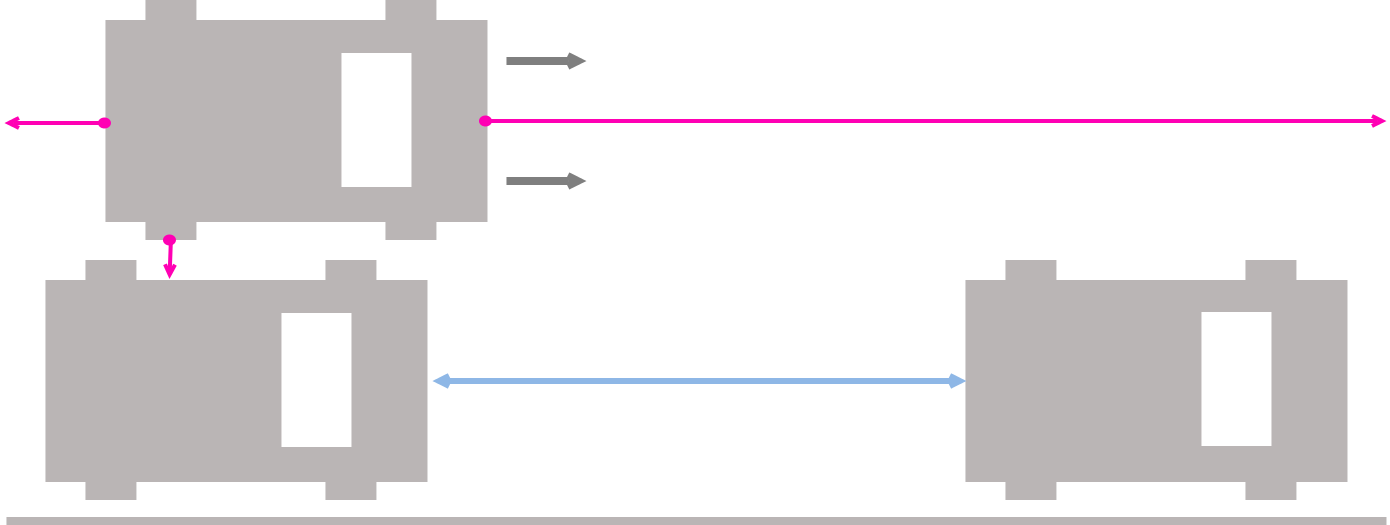
\includegraphics[width=0.8\textwidth]{david_images/Problem.png}
  		\caption{\tiny Car needs to autonomously pass by the parking lot, detect it and perform a parallel parking maneuver}
	\end{figure}
  \end{frame}

  \subsection{Algorithm}
  \begin{frame}{Basics}
  	\begin{itemize}
  	\item<1-> calculation of actuator data
  		\begin{itemize}
  		 \item<2-> velocity v
  		 \item<3-> steering angle $\phi$
  		\end{itemize}
  	\item<4-> no computation of an exact path
  	\item<5-> actuator data is determined by the evaluation of our 3-phase algorithm
  	\end{itemize}
  \end{frame}

  \begin{frame}{Phase 1 - Searching phase (1)}
  	\begin{figure} [ht]
  		\centering
  		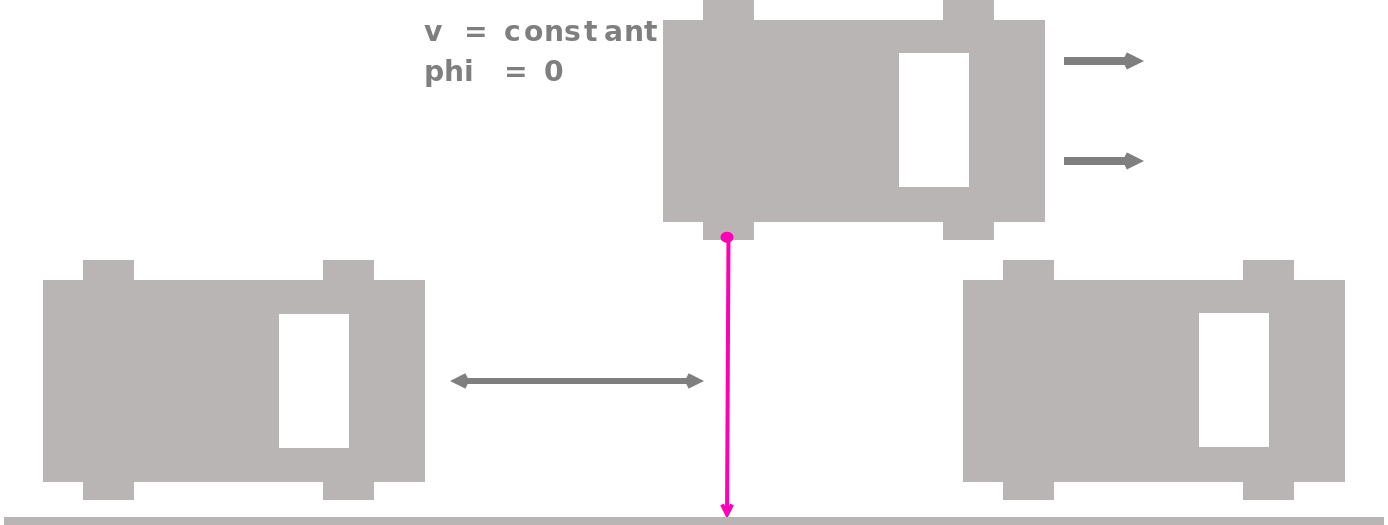
\includegraphics[width=1.0\textwidth]{david_images/FindLot1.png}
  		\caption{\tiny Car passes the potential parking lot and calculates its size}
	\end{figure}
  \end{frame}

  \begin{frame}{Phase 1 - Searching phase (2)}
  	\begin{figure} [ht]
  		\centering
  		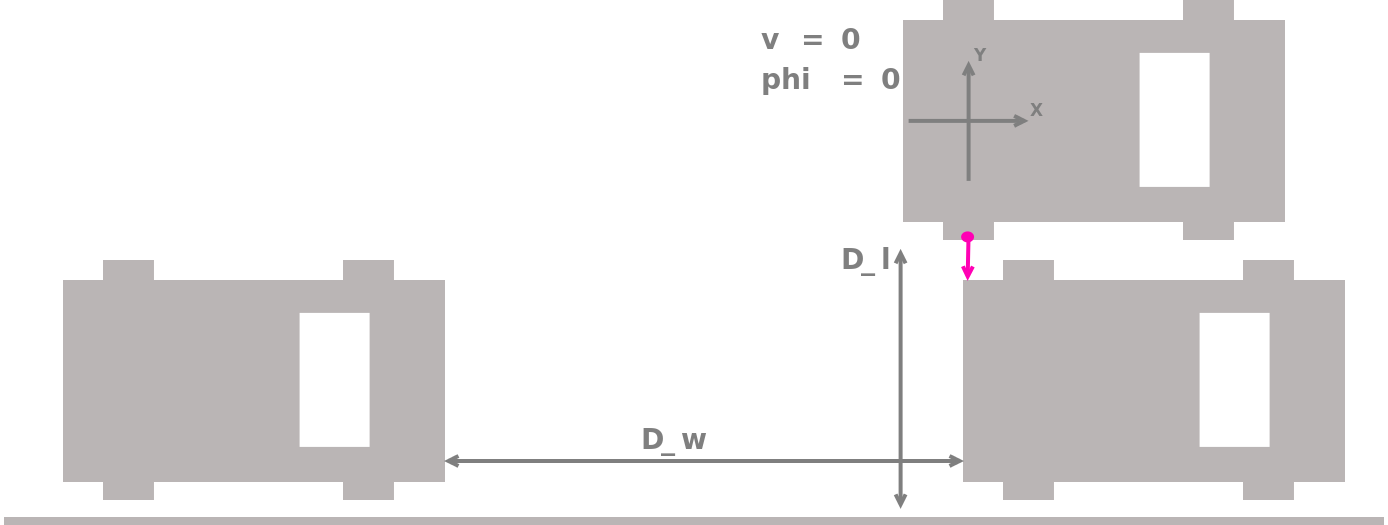
\includegraphics[width=0.9\textwidth]{david_images/FindLot2.png}
  		\caption{\tiny Algorithm creates environment and position information}
	\end{figure}
  \end{frame}

  \begin{frame}{Phase 2 - Calculation phase (1)}
    	\begin{itemize}
  		\item<1-> equations of vehicle's motion:
  			\begin{itemize}
  				\item<2-> $\dot{x} = v * cos(\phi) * cos(\theta)$
  				\item<3-> $\dot{y} = v * cos(\phi) * sin(\theta)$
  				\item<4-> $\dot{\theta} = \frac{v}{L} * sin(\phi)$
  			\end{itemize}
  		\item<5-> time dependant formulas for v and $\phi$ needed
  			\begin{itemize}
  				\item<6-> $\phi(t)$ - steering angle (based on max $\phi$)
  				\item<7-> $v(t)$ - velocity (based on max v)
  			\end{itemize}
  		\item<8-> time for whole menauever is estimated and optimized
  	\end{itemize}
  \end{frame}

  \begin{frame}{Phase 2 - Calculation phase (2)}
  	\begin{figure} [ht]
  		\centering
  		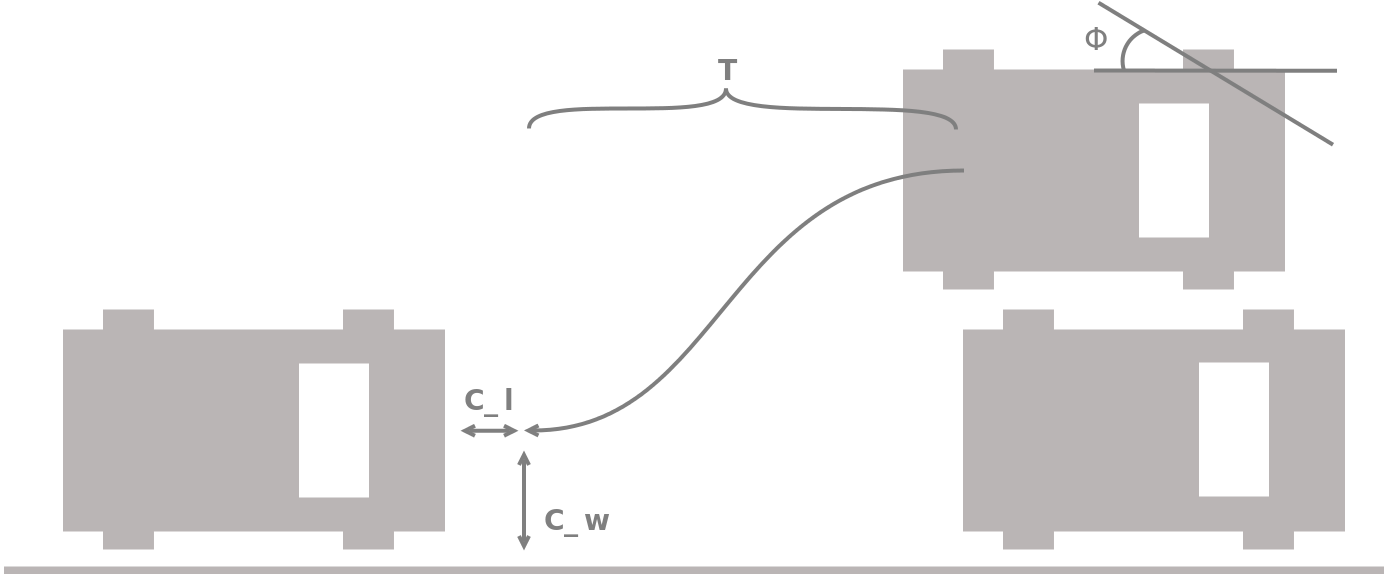
\includegraphics[width=0.9\textwidth]{david_images/Calculating.png}
  		\caption{\tiny Algorithm simulates parking maneuver to calculate duration and steering angle}
	\end{figure}
  \end{frame}

  \begin{frame}{Phase 3 - Parking phase}
  	\begin{figure} [ht]
  		\centering
  		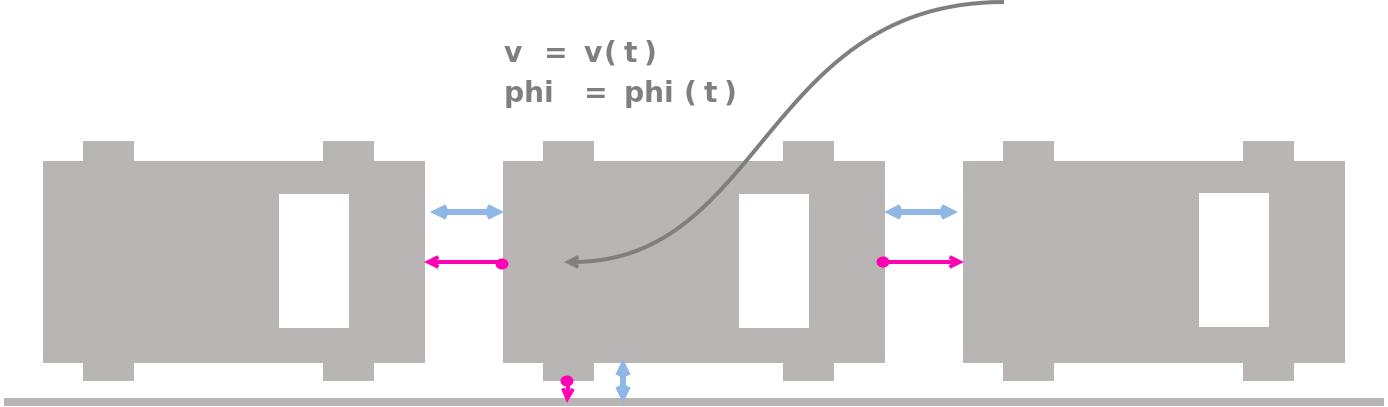
\includegraphics[width=0.9\textwidth]{david_images/Parked.png}
  		\caption{\tiny Algorithm steers and accelerates the car according to calculation until parking position is reached}
	\end{figure}
  \end{frame}

  \subsection{Problems and Limitations}
  \begin{frame}{Problems and Limitations}
  	\begin{itemize}
  		\item<1-> calculation of parking duration is based on magic number
  		\item<2-> longitudinal and lateral distance conditions seem to work not properly
  		\item<3-> safety distance needs to be higher than necessary
  	\end{itemize}
  \end{frame}

\section{Summary}
\againframe<all:8>{ourtask}

\end{document}
